\section{IMPLEMENTATION DETAILS}
\label{app:implementation}

\subsection{Architecture and Hyperparameters}
\label{app:architecture}

\cref{tab:architecture} lists every network and every fixed quantity as implemented; the weights marked calibrated are set per section by the protocol of \cref{sec:invariance} and are not quoted here. All multilayer perceptrons use rectified-linear hidden units.

\begin{table}[t]
\centering
\caption{Networks and fixed quantities. $G$ genes, $K$ types, $\dPhi$ image-embedding dimension.}
\label{tab:architecture}
\small
\begin{tabular}{@{}p{0.2\textwidth}p{0.27\textwidth}p{0.48\textwidth}@{}}
\toprule
Component & Input & Layers / value \\
\midrule
Count encoding & $\vx_i$ & $[\log(1 + \vx_i \tilde\ell/\ell_i),\ \log\ell_i]$, $\tilde\ell$ the median total \\
$q(\vz_i \mid \vx_i, t_i)$ & count encoding $\oplus \onehot(t_i)$ & $256 \to 256 \to 2\dz$, $\dz = 20$ \\
Type query $\embed(t_i)$ & $t_i$ & learned table, width $K$ \\
Attention sources & neighbour $j$ & $\onehot(t_j)$, width $K$; an earlier version appended the neighbour's posterior mean under a stop-gradient and was dropped after a three-seed ablation \\
Attention layer & sources, query & one bipartite GATv2 layer, $4$ heads $\times\, 32$, averaged, LeakyReLU slope $0.2$, no self-loops, no edge features \\
Context $\vc_i$ & & attention output ($32$) $\oplus\ \vPhi_i$ ($\dPhi = 384$) $\oplus$ isolation flag ($1$) \\
Prior mean $\mpsi(\vc_i, t_i)$ & $\vc_i \oplus \onehot(t_i)$ & $64 \to \dw$, $\dw = 6$ \\
$q(\vw_i \mid \cdot)$ & $\vc_i \oplus \onehot(t_i) \oplus \vz_i \oplus$ count encoding & $256 \to 2\dw$ \\
Decoder $a(\vz_i)$ & $\vz_i$ & $256 \to G$ \\
Loadings $\vB$ & $\vw_i$ & linear $\dw \to G$, no bias \\
Adversary heads & $\vmu_{z,i} \oplus \onehot(t_i)$ & two heads $64 \to 64 \to K$ (composition) and $\to \Ephi = K$ (image niche) \\
Image niche $\ephi_i$ & $12$ principal components of $\vPhi$ & soft $k$-means memberships $\softmax(-d^2/T)$, $T$ the median nearest squared distance; the projection is fitted on a $50{,}000$-cell random subsample and applied to all cells, the $k$-means (four restarts) on all cells; fitted once and frozen \\
Invariance block $\vv_i$ & & $[\vy_i^{(-K)},\ 12 \text{ principal components of } \vPhi_i]$ \\
Held-out probes & $\vmu_{z,i} \oplus \onehot(t_i)$ & ridge regression ($\lambda = 10^{-3}$) and perceptron $64 \to 64$ ($300$ Adam steps at $10^{-3}$, batches of $2{,}048$), each scored per block against its own within-type permutation floor; both fitted on at most $30{,}000$ training-tile cells \\
\midrule
Graph & & Delaunay adjacency; Voronoi faces measured within $30\um$ discs; prune at $40\um$ \\
Kernel $\beta$ & & $f_{ij}\exp(-d_{ij}/\tau)$, $\tau = 20\um$, row-normalised over in-edges \\
Prior scale $\sigma_w$ & & $1$ (fixed) \\
\midrule
Leak fraction $\kappa$ & & swept over $\{0, 0.05, 0.1, 0.2, 0.3, 0.4\}$; the operating point $0.1$ is a grid point chosen on the primary section (\cref{sec:setup}) \\
$\omega$ & & $1$ \\
$\alphaz$ & & $\tfrac12/\lbar$, half the bound-equivalent value, with $\lbar$ the section's count scale (\cref{sec:objective}) \\
$\alphaw$ & & $0.1$, far above $1/\lbar$ (\cref{sec:objective}); ramped linearly from $0$ over the first $30$ epochs \\
$\alphaa$ (adversary) & & $0.3$; six head updates per model update at learning rate $2 \times 10^{-3}$, set so that the independent probe, not the heads' own loss, certifies head strength; composition half weighted $\lambda_y = 3$ \\
$\alphaa$ (closed form) & & calibrated by the same probe protocol \\
Moving-average rate, shrinkage & & $0.05$, $0.05$; support floor $10\times$ joint dimension \\
\midrule
Tiles & & recursive median split into rectangles of $\leq 4{,}096$ cells; $15\%$ of tiles held out \\
Optimiser & & Adam \citep{kingma2015adam}, learning rate $10^{-3}$, cosine annealing \citep{loshchilov2017} over the epoch budget, gradient-norm clip $10$ \\
Evaluation & & every $5$ epochs on posterior means; checkpoint accepted if held-out reconstruction improves and $\vz$--type agreement $\geq 0.9\times$ its running maximum; patience in epochs set with the budget; $\alphaw$ ramped linearly from $0$ over the first $30$ epochs, during which no checkpoint is accepted and patience does not count \\
Hardware & & one NVIDIA GeForce RTX 4090 (24\,GB) per fit \\
\bottomrule
\end{tabular}
\end{table}

\subsection{Choices Made in Implementation}
\label{app:deviations}

Where the model description of \cref{sec:method} leaves a choice open, \cref{tab:deviations} records what was done and why. Every entry is also stated in the method text; the table collects them in one place. \todo{author to decide whether this table stays; it duplicates the method text}

\begin{table}[t]
\centering
\caption{Implementation choices and their reasons.}
\label{tab:deviations}
\small
\begin{tabular}{@{}p{0.22\textwidth}p{0.36\textwidth}p{0.36\textwidth}@{}}
\toprule
Where & Decision & Reason \\
\midrule
Type input to $q(\vw)$ and $\mpsi$ & one-hot everywhere the type is an input; the learned type embedding exists only as the attention query, sized to match the source features & the query stands in for the $\vz_i$ that the cell deliberately does not contribute to its own context \\
Counts input to $q(\vw)$ & the same encoding as $q(\vz)$ & one encoding of the counts for both posteriors \\
Neighbour responses $\vw_j$ & a posterior draw from the same batched pass, under a stop-gradient & the neighbours' clean compositions must include their local programme (\cref{sec:batching}) \\
Invariance block & one composition column dropped & the simplex makes the full block singular; the information is unchanged (\cref{app:gaussian-mi}) \\
Penalty matrices & correlation rather than covariance form, plus $10^{-5}\vI$ on the correlation matrix before the log-determinant & identical value by scale invariance; bounded gradient; on a unit-diagonal matrix the additive term is a uniform relative jitter, not a variance-inflating ridge \\
Penalty gradient & straight-through: value from the moving averages, gradient from the batch & otherwise the effective strength of $\alphaa$ scales with the averaging rate \\
Penalty, adversary and probe input & posterior means $\vmu_z$, not samples & encoder noise would dilute the measured dependence \\
Objective granularity & per-cell mean over the batch rather than a sum & invariant to tile size \\
Evaluation draws & posterior means & the stopping signal should not ride reparameterisation noise \\
Image embedding dimension & the full native embedding into $\vc_i$ rather than a $32$--$64$-dimensional projection & the deciding test is held-out reconstruction with and without the projection; the invariance block uses $12$ principal components regardless \\
Probe target for the image & Gaussian log-likelihood gain on the continuous components, per block, rather than categorical cross-entropy against image-niche clusters & the closed-form penalty takes continuous components directly; a small nonlinear probe is fitted alongside and is the probe the decision rule reads (\cref{sec:invariance}) \\
Graph construction & the Voronoi tessellation is clipped to $30\um$ discs before faces are measured, then edges are pruned at $40\um$ & the clip removes faces only for pairs more than roughly $60\um$ apart, which the prune removes anyway, and bounds the length of faces at tissue borders and across gaps; the effect on $\beta$ for kept edges has not been quantified \todo{quantify} \\
Invariance mechanism & the adversary is the operating configuration; the closed-form penalty is the cheaper first attempt & the escalation rule of \cref{sec:invariance} decides between them on each section \\
\bottomrule
\end{tabular}
\end{table}

\begin{table}[t]
\centering
\caption{Implementation choices, continued: the configuration used in the experiments, and what exists but is switched off.}
\label{tab:deviations2}
\small
\begin{tabular}{@{}p{0.22\textwidth}p{0.36\textwidth}p{0.36\textwidth}@{}}
\toprule
Where & Decision & Reason \\
\midrule
Attention sources & neighbour types only; an earlier version also passed the neighbour's posterior mean under a stop-gradient & the case is empirical, not mechanistic: a seed-matched ablation improved held-out reconstruction, the $\vz$--type agreement, the mirror check and the cycle readout of $\vw$ while leaving $\vw$'s spatial readouts unchanged. The mechanism originally proposed for it, the prior reconstructing a cell from its neighbours' codes, was tested with two purpose-built detectors and not confirmed; the sources are types because the ablation is better, not because that mechanism was demonstrated \\
Training budget & two budgets: a short one for sweep points, a long one for reference fits (\cref{sec:selection}) & sweep points must be comparable to one another; reference fits must be individually good, and the better optimisation basin is not reached at the short budget \\
Choosing among seeds & several seeds per reference configuration, one selected on the full diagnostic battery, the rest reported as the envelope & selection on held-out reconstruction alone admits a fit that buys likelihood at the cost of the intrinsic-state readouts \\
Halo overhead & ring one is fully encoded; ring two contributes a type lookup only & the attention sources are types, so ring two needs no encoder pass and none is run; the node overhead falls with tile size, and tiles are sized above the knee \\
Resident count storage & the count matrix is held on the accelerator as $16$-bit integers and cast per tile & counts are small non-negative integers, so the narrow type is exact and is asserted to be; the wide type does not fit on one consumer card for the largest section, and tile size does not help, since every tile is resident \\
\midrule
Built but not default & leak-subtracted encoder input $\tilde\vx_i = \max(\vx_i - \kappa\ell_i\rhobar_i, 0)$, normalised by its own total with the log-depth scalar left raw, as the counts-level answer to the amortisation gap; an attention sink, a fixed null logit joining every destination's softmax so that the aggregate saturates in the number of neighbours instead of ignoring it; coupled weight decay in the optimiser & each is available behind a flag and off in every fit reported here. The encoder correction is retained as an ablation rather than as the model, since it changes the evidence $\vz$ is formed from; the sink cannot be exercised on a Delaunay graph, whose degree is nearly constant, and is kept for graphs whose degree varies; weight decay is recorded because it moves the gauge of \cref{sec:sweep} rather than removing it \\
\midrule
Not built & Dirichlet-multinomial likelihood; per-cell counterfactuals with abduction; bounded conditional $\sigma_w(\vc,t)$; estimation of $\kappa$ from a nuclear/extranuclear split; edge features in the attention layer & each has a stated trigger that has not fired, or is future work. The \emph{type-level} counterfactual, in which the context prior is moved between two neighbourhoods with the intrinsic state held fixed, is built and exercised; only the per-cell form, which needs a non-degenerate response posterior, is not \\
\bottomrule
\end{tabular}
\end{table}

\subsection{Tiles and the Two-Hop Halo}
\label{app:tiles}

\Cref{fig:batching} shows the tiles, the held-out split and the halo of one training tile on the primary section, as built for a fit (\cref{sec:batching}).

\begin{figure}[t]
\centering
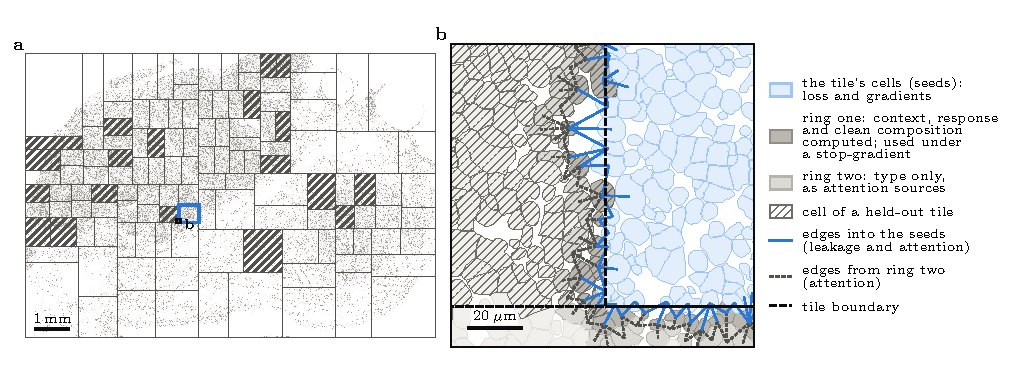
\includegraphics[width=\textwidth]{figures/fig_batching}
\caption{Tiles, the held-out split and the two-hop halo on the primary section. \textbf{a},~The section cut into contiguous tiles of at most $4{,}096$ cells by recursive median split. Hatched tiles are held out ($15\%$ of tiles, one split). The blue tile is shown in b, and the black square marks the window of b. \textbf{b},~Where that training tile meets a held-out tile (left) and another training tile (below). The tile's cells are the seeds, on which the loss is evaluated. Ring one, their graph neighbours, has its context, response and clean composition computed in the same pass. Those compositions enter the seeds' foreign influx under a stop-gradient, and ring one's types are attention sources for the seeds (solid edges). Ring two, the neighbours of ring one, contributes only its types, as attention sources for ring one (dashed edges). Both rings are read from the leakage kernel's own edge list. Hatched cells belong to the held-out tile: ring cells drawn from it enter training as inputs, with no loss and no gradient (\cref{sec:batching}).}
\label{fig:batching}
\end{figure}

\subsection{The Held-Out Probe}
\label{app:probe}

\Cref{fig:probe} shows how the probe of \cref{sec:invariance} is fitted, scored and read.

\begin{figure}[t]
\centering
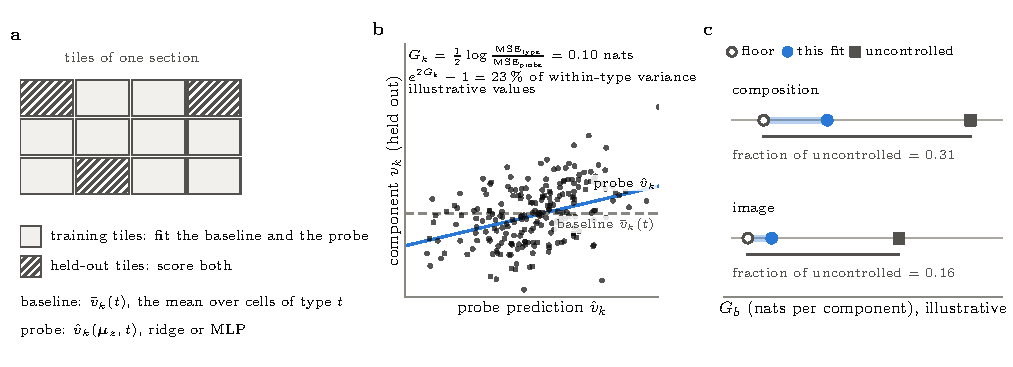
\includegraphics[width=\textwidth]{figures/fig_probe}
\caption{How the held-out probe grades the invariance of $\vz$ (\cref{eq:probe}); schematic, with synthetic values chosen for legibility. \textbf{a},~The type-only baseline and the probe are fitted on the training tiles and scored on the held-out tiles (hatched). The baseline predicts each component of the invariance block by its mean over cells of the same type; the probe predicts it from $(\vmu_z, t)$ with a ridge regression or a small perceptron. \textbf{b},~One component for held-out cells of one type. The baseline's error is the spread around the type mean (dashed), the probe's the spread around its prediction (solid, the line of perfect prediction). $G_k$ is half the log ratio of the two mean squared errors, $e^{2G_k} - 1$ is the share of within-type variance the probe explains, and $G_b$ averages $G_k$ over the block. \textbf{c},~Reading $G_b$ for each block. The floor is its value with $\vmu_z$ permuted within type; the uncontrolled fit is the same model with $\alphaa = 0$. What is reported is this fit's excess over the floor (blue bar) and that excess as a fraction of the uncontrolled fit's (grey bracket), for each probe family. A block passes when that fraction is at most a quarter (dotted guard): here the composition block fails and the image block passes.}
\label{fig:probe}
\end{figure}

\Cref{tab:probe} gives the probe on the final fits of every section.

\begin{table}[t]
\centering
\caption{The held-out probe on the final fits, per section. For each block, the share of its within-type variance that the probe explains from $\vz$ beyond the permutation floor ($e^{2\,\mathrm{excess}} - 1$, in \%), for the model trained without the adversary ($\alphaa = 0$, two seeds) and with it (the final fits, three seeds), the largest share with the adversary that would pass (\emph{needed to pass}: a quarter of the excess without the adversary, as a share), and the quantity the guard reads, the \emph{fraction left}: the excess with the adversary as a fraction of the mean excess without it, $0$ when the adversary removes everything the probe can find and $1$ when it removes nothing. Ranges are over seeds. A seed passes when all four fractions (two blocks, two probes) are at most a quarter. The sections end at a similar absolute residual; the fraction left is larger where less leaked to begin with. Section B of the lung TMA is graded with the models fitted on section A. \pending{regenerate once Unassigned is excluded as a target in the re-read of the final fits}}
\label{tab:probe}
\small
\setlength{\tabcolsep}{5pt}
\begin{tabular}{@{}lccccc@{}}
\toprule
& Ovarian FFPE & Lung FFPE & Ovarian FF & Lung TMA A & Lung TMA B \\
\midrule
\multicolumn{6}{@{}l}{\emph{Composition, MLP probe}} \\
\quad without the adversary (\%) & 19.5--20.8 & 11.8--12.4 & 36.3--37.4 & 5.5--7.0 & 6.8--7.0 \\
\quad with the adversary (\%) & 4.4--5.7 & 3.9--4.7 & 4.4--4.9 & 3.1--4.4 & 3.9--4.6 \\
\quad needed to pass (\%) & 4.7 & 2.9 & 8.2 & 1.5 & 1.7 \\
\quad \textbf{fraction left} & \textbf{0.23--0.30} & \textbf{0.33--0.40} & \textbf{0.14--0.15} & \textbf{0.50--0.71} & \textbf{0.58--0.67} \\
\addlinespace
\multicolumn{6}{@{}l}{\emph{Image, MLP probe}} \\
\quad without the adversary (\%) & 14.8--17.1 & 9.5--10.9 & 34.3--37.0 & 5.8--8.3 & 5.3--7.2 \\
\quad with the adversary (\%) & 2.5--4.1 & 1.4--2.0 & 4.5--4.9 & 2.2--2.8 & 2.0--3.0 \\
\quad needed to pass (\%) & 3.8 & 2.5 & 7.9 & 1.7 & 1.5 \\
\quad \textbf{fraction left} & \textbf{0.17--0.27} & \textbf{0.14--0.20} & \textbf{0.14--0.16} & \textbf{0.32--0.40} & \textbf{0.32--0.49} \\
\addlinespace
\multicolumn{6}{@{}l}{\emph{Ridge probe, fraction left}} \\
\quad composition & 0.16--0.23 & 0.15--0.19 & 0.07--0.08 & 0.19--0.22 & 0.32--0.45 \\
\quad image & 0.08--0.16 & 0.05--0.16 & 0.10--0.13 & 0.19--0.21 & 0.17--0.39 \\
\midrule
Seeds passing & 1/3 & 0/3 & 3/3 & 0/3 & 0/3 \\
\bottomrule
\end{tabular}
\end{table}

